
    %%%%% %%%%% %%%%%
    %               %
    % New row       %
    %               %
    %%%%% %%%%% %%%%%
\begin{columns}[t]
  \begin{column}{0.65\textwidth}
    \begin{block}{\large Windowing}
      \begin{columns}
        \begin{column}{0.68\textwidth}
%\small
\footnotesize
%\tiny
Allele balance can also be used to assign copy number to genomic windows of variants.
Windows of user specified lengths can be made and allele balance is estimated for each window.
A distance from expectation and the number of heterozygous position for each window are reported to help determine the quality of estimates.
Estimates determined to be of low quality may be censored.
        \end{column}
        \begin{column}{0.30\textwidth}
          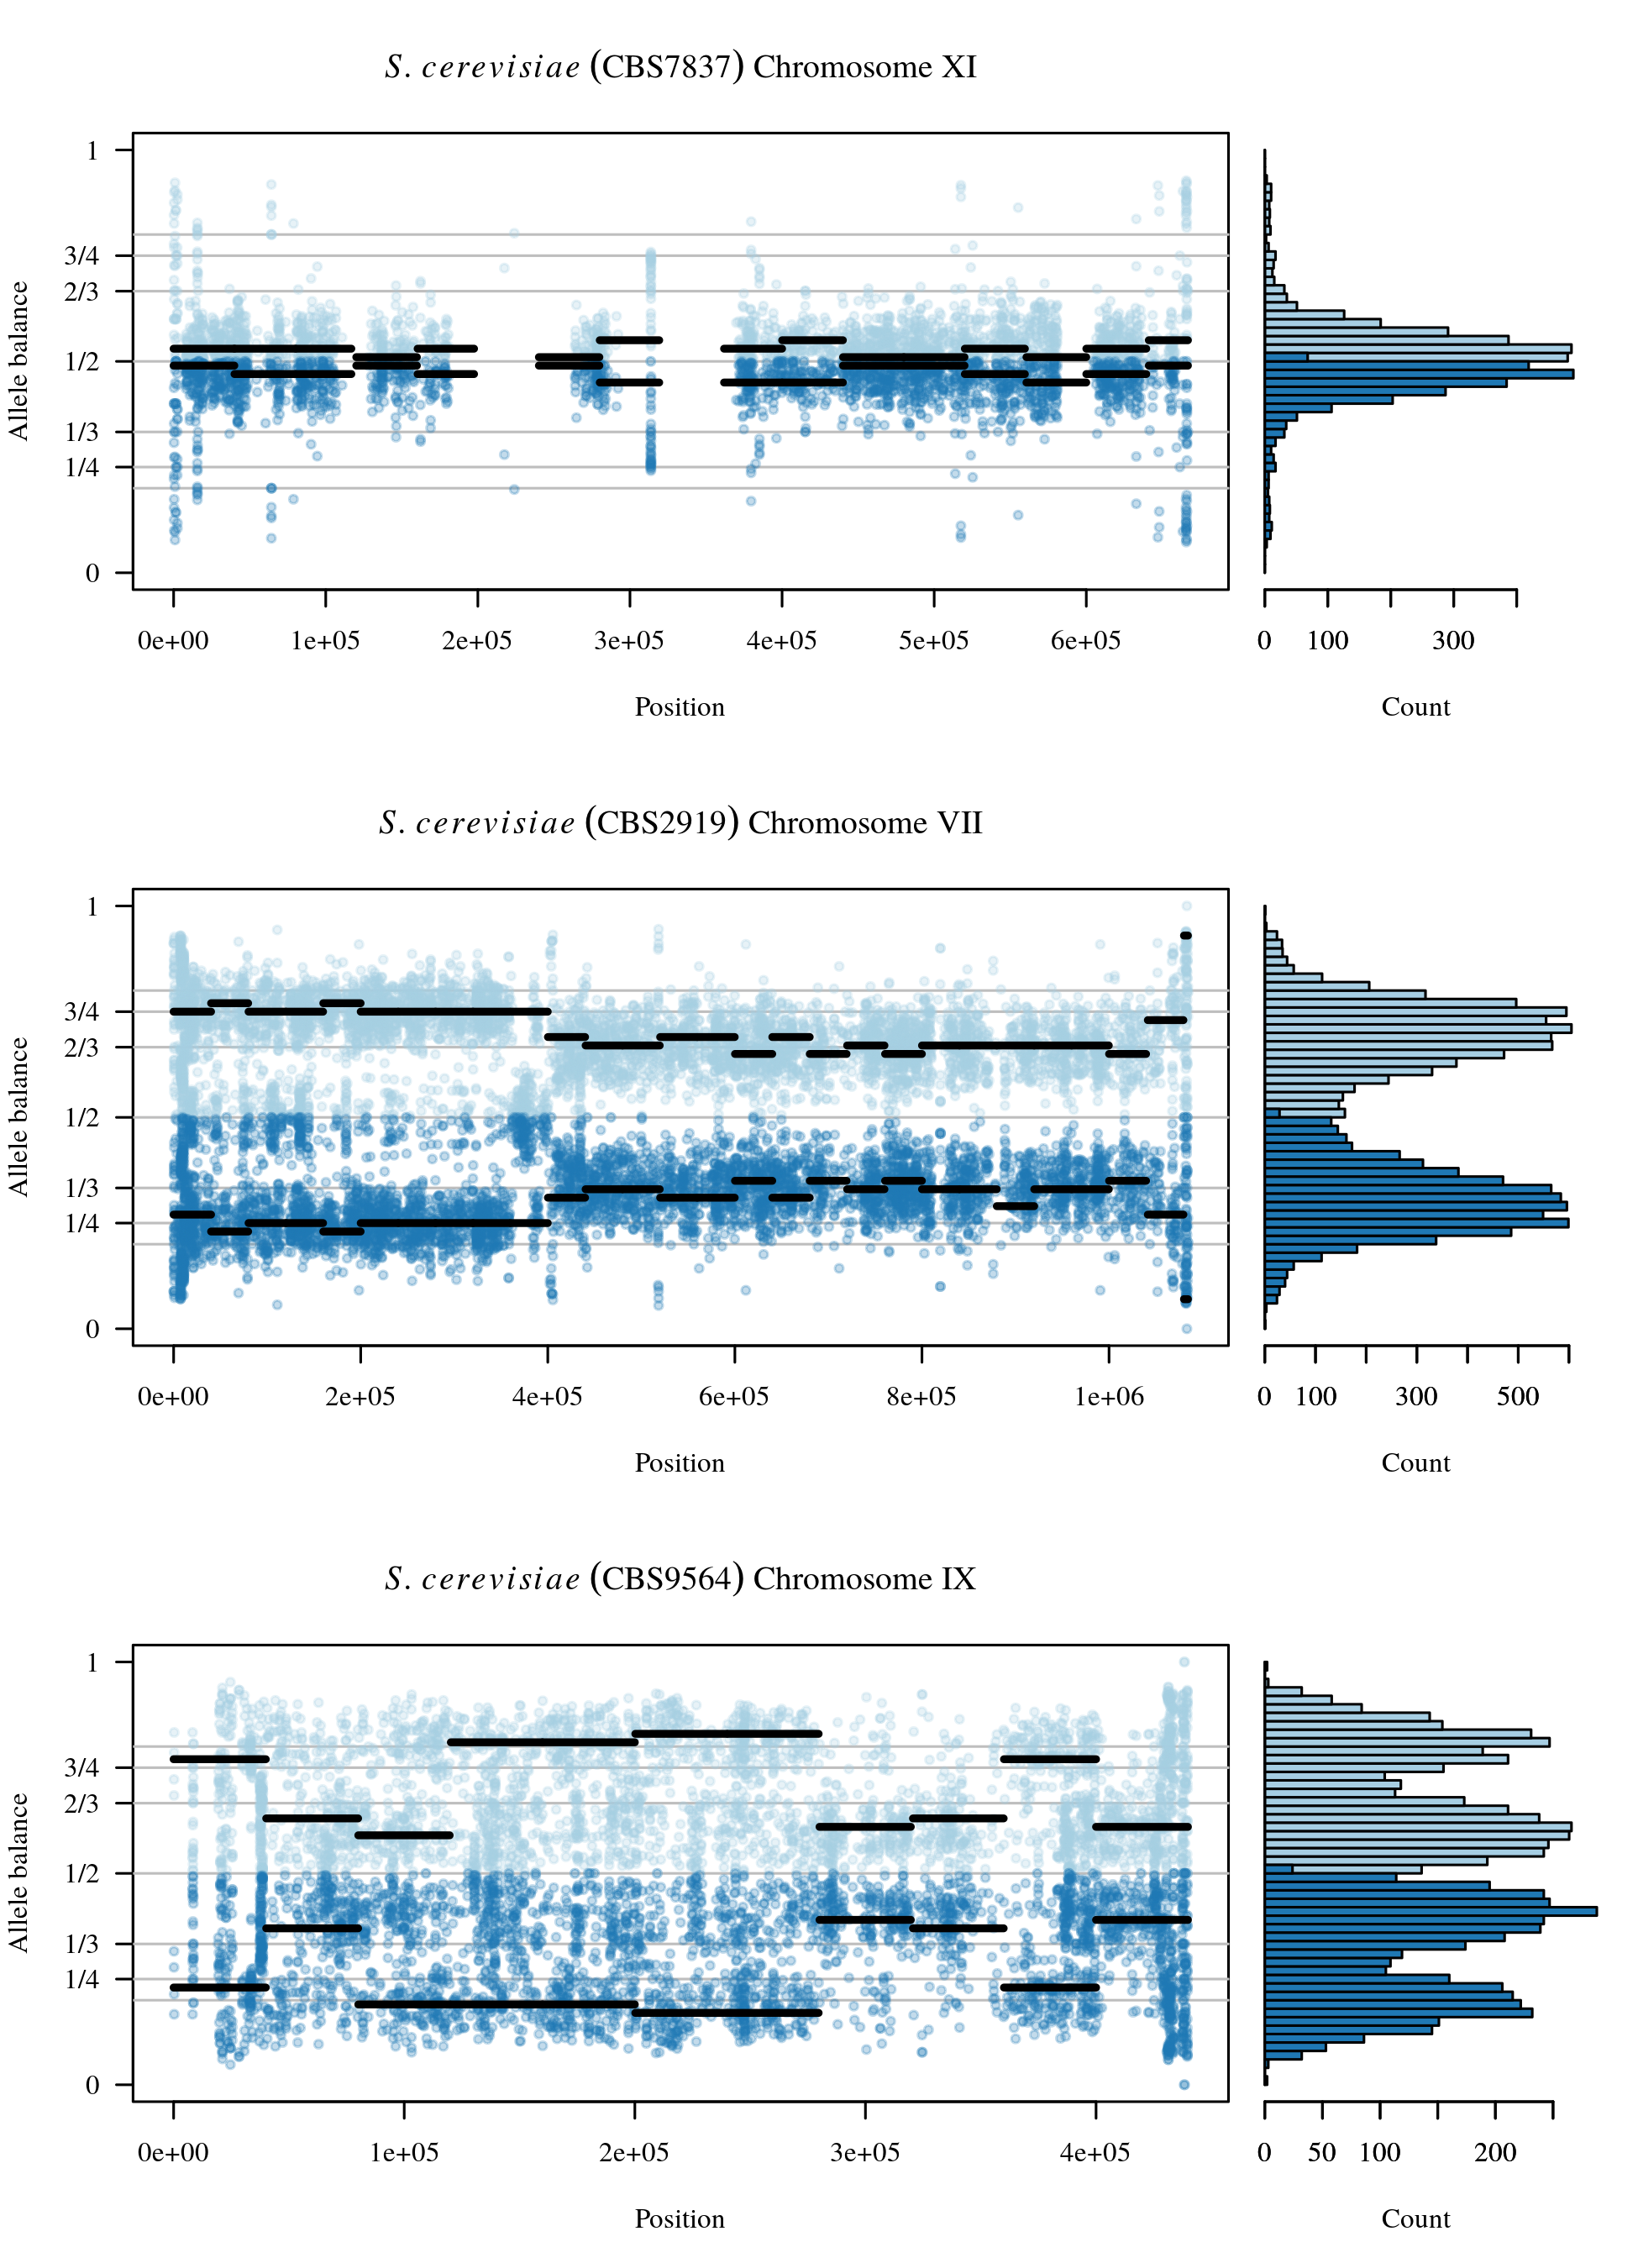
\includegraphics[height=20cm]{./figures/fig6_exemplars.png}
        \end{column}
      \end{columns}

    \end{block}
  \end{column}

  \begin{column}{0.32\textwidth}
    \begin{block}{\large Acknowledgments}
\tiny
\vspace{5mm}

This research is supported in part by U.S. Department of Agriculture (USDA) Agricultural Research Service Grant 5358-22000-039-00D and USDA National Institue of Food and Agriculture Grant 2011-68004-30154.
\newline
\vspace{10mm}

\textit{Saccharomyces cerevisiae} data from:
Zhu YO, Sherlock G, Petrov DA. 
Whole genome analysis of 132 clinical \textit{Saccharomyces cerevisiae} strains reveals extensive ploidy variation.
G3. 2016; 6(8):2421-34. https://doi.org/10.1534/g3.116.029397.
\newline
\vspace{10mm}

vcfR can be found at:
https://CRAN.R-project.org/package=vcfR

\vspace{15mm}

    \end{block}
  \end{column}
\end{columns}


